%% May 2016, 
%presentation inspired by the presentation made in CAA, the presentation made at the Winter Simulation Conference, and some ideas tooks from #RIN4 at the UPF

\documentclass[12pt, notes=show]{beamer}
\usetheme[width=0cm]{Goettingen}
\usecolortheme{rose}
\useoutertheme{default}
\setbeamerfont{caption}{size=\scriptsize}
\setbeamertemplate{navigation symbols}{}

\addtobeamertemplate{navigation symbols}{}{%
	\usebeamerfont{footline}%
	\usebeamercolor[fg]{footline}%
	\hspace{1em}%
	$\dfrac{\insertframenumber}{\inserttotalframenumber}$
}

\usepackage{fontspec} 
\setsansfont{Futura LT}



\title{
	Cultural evolution and long term economic dynamics :\\The case study of Rome.
}

\institute{May 2016}

\author{Simon Carrignon\\\vspace{.5cm} {\tiny Supervisors: Xavier Rubio-Campillo \& Sergi Vavlerde}}

\date{
	\scriptsize
	\begin{columns}
		\begin{column}{.3\textwidth}
			\begin{center}
				Barcelona Supercomputing Center	\\
				
\includegraphics[height=1cm]{images/bscLogo.jpg} \hspace{2cm}
			\end{center}
		\end{column}
		\begin{column}{.3\textwidth}
			\begin{center}
				Univ. Pompeu Fabra Complex System Lab.\\
				\includegraphics[height=1cm]{images/upfLogo.jpeg} %declare logo image with an alias here 
			\end{center}
		\end{column}
	\end{columns}

}
\begin{document}
\begin{frame}
	\maketitle

\end{frame}

\section{Methods}
\begin{frame}
    \centering
    \Large
   Institutions 
\end{frame}
\begin{frame}{Context}
    \vfill
    \begin{description}
	\item[School:] UPF PhD Programme in Biomedicine 
    \vfill
	\item<2->[Supervision:] Xavier Rubio (BSC) \\ Sergi Valverde (UPF-Complex System Lab)
    \vfill
	\item<3->[Funding:] 4-years grant from EPNet project \\ (ERC advanced Grant 340828):
    \end{description}
    \vspace{-.2cm}
    \uncover<3->{\begin{quote}
	\small
	Production and Distribution of Food during the Roman Empire: Economic and Political Dynamics
    \end{quote}}
    \vfill
\end{frame}

\section{Introduction}

\begin{frame}
    \centering
    \Large
    General Question
\end{frame}
\begin{frame}{Cultural Evolution}
    Social Traits:
    \begin{center}
	\begin{table}
	    \center
	    \begin{tabular}{ccc}
		\uncover<2->{\includegraphics[height=3cm]{images/m80}} &
		\uncover<3->{\includegraphics[height=3cm]{images/m90}} &
		\uncover<4->{\includegraphics[height=3cm]{images/m10}} \\
		\uncover<2->{80's} & \uncover<3->{90's} & \uncover<4->{now}
	    \end{tabular}
	\end{table}
    \end{center}
    \uncover<5->{How they Evolve?}\uncover<6>{ Cultural Evolution }
\end{frame}

\begin{frame}{Cultural Evolution}
    \begin{itemize}
	\item<5->{ culturally transmitted, socially learnt}
	\item<6->{ similar patterns}
    \end{itemize}
	\begin{center}
		\uncover<4->{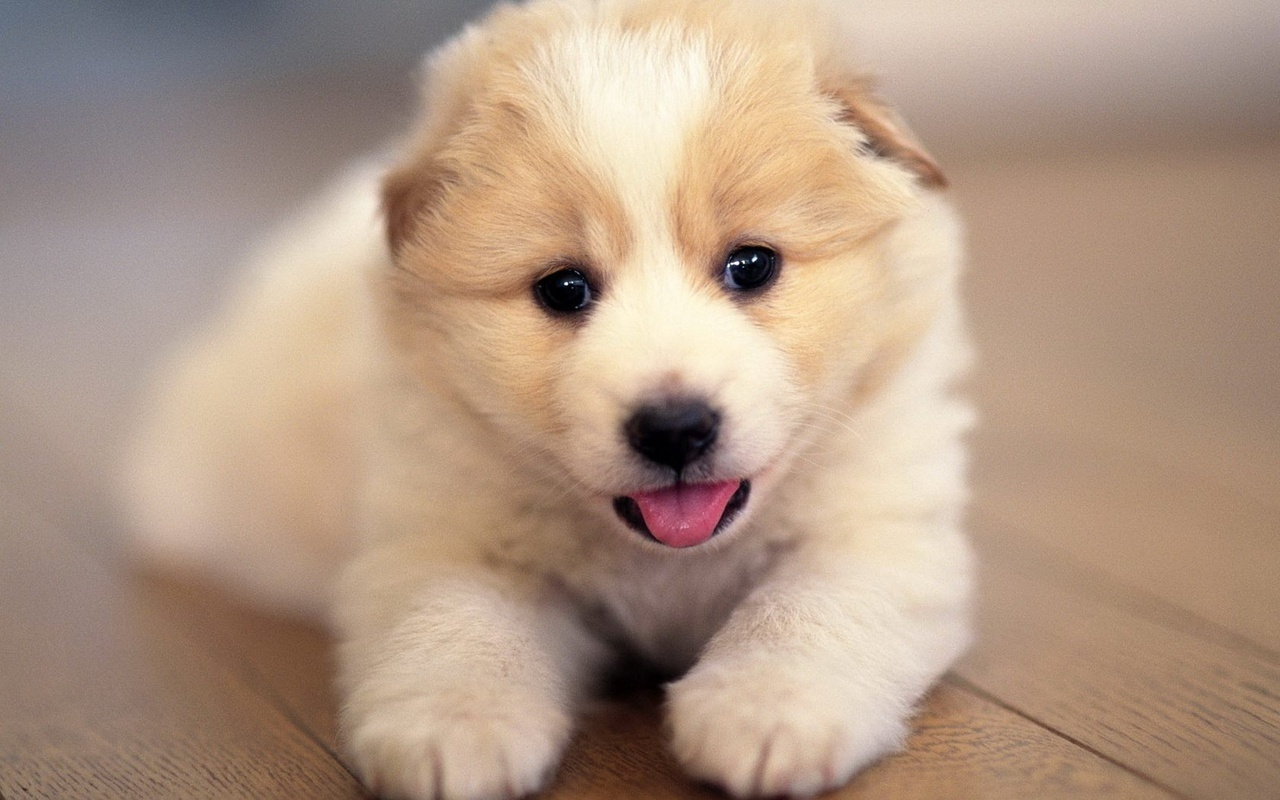
\includegraphics[width=3cm]{images/cutdog}}\\
		\vspace{.5cm}
		\uncover<2->{\includegraphics[width=2.5cm]{images/cutbaby}}
	    \hspace{1cm}
	    \uncover<3->{ \includegraphics[width=2cm]{images/pottery}}
	\end{center}
    \uncover<7>{$\rightarrow$ What mechanism drive the evolution of such traits?\\
    \invisible<1->{$\rightarrow$ What mechanism }generate such pattern?}
\end{frame}

\begin{frame}{What Generate Those Cultural changes?}
	Simple mechanisms (Bentley et al, 2004):
	\begin{itemize}
		\item<2->Random Copy 
		\item<3-> Frequency biased (conformist/anti-conformist\dots)
		\item<4->\dots	
	\end{itemize}
	\uncover<2>{\begin{figure}
		\begin{columns}
			\begin{column}{.8\textwidth}
				\centering
				\includegraphics[width=.6\textwidth]{images/powerlawrepartition.jpg}
			\end{column}
			\begin{column}{.3\textwidth}
				\tiny
				Square: male names\\
				Circle: female names\\
				Dotted and plain lines: model result with different copy probabilities.\\
			From Bentley et al,~2004.
			\end{column}
		\end{columns}
	    \end{figure}}
\end{frame}


\section{Scientific Context}

\begin{frame}
	\begin{center}
	    What if such mechanisms act on traits linked to economics?
	\end{center}
	\begin{center}
	    \only<2>{\vspace{1cm}\includegraphics[height=3cm]{images/bordeaux.jpg}\hspace{2cm}
	    \includegraphics[height=3cm]{images/napa}}
	    \only<3>{\includegraphics[height=4cm]{images/tools}}
	    \only<4>{\includegraphics[height=4cm]{images/stockoption}}
	\end{center}
\end{frame}

%
\begin{frame}{Co-evolution of Economy and Culture}

    \begin{center}
	\includegraphics[width=\textwidth]{images/interaction}	
    \end{center}

\end{frame}



\section{Methods}
\begin{frame}
    \centering
    \Large
    Approach
\end{frame}


\begin{frame}{Approach}
    \begin{itemize}
	\item Archaeology
	    \begin{itemize}
		\item<3-> Compare culture across time (vs ``twitter studies'')
	    \end{itemize}
	    \vfill
	\item<2-> Computer Simulation
	    \begin{itemize}
		\item<4-> Compare \& Select models
		\item<5-> Explore \& Generate hypothesis
	    \end{itemize}
	    \vfill
    \end{itemize}
\end{frame}

\begin{frame}
    \begin{center}
	\includegraphics[width=\textwidth]{images/approach.pdf}		
    \end{center}
    
\end{frame}

\begin{frame}
    \begin{center}
	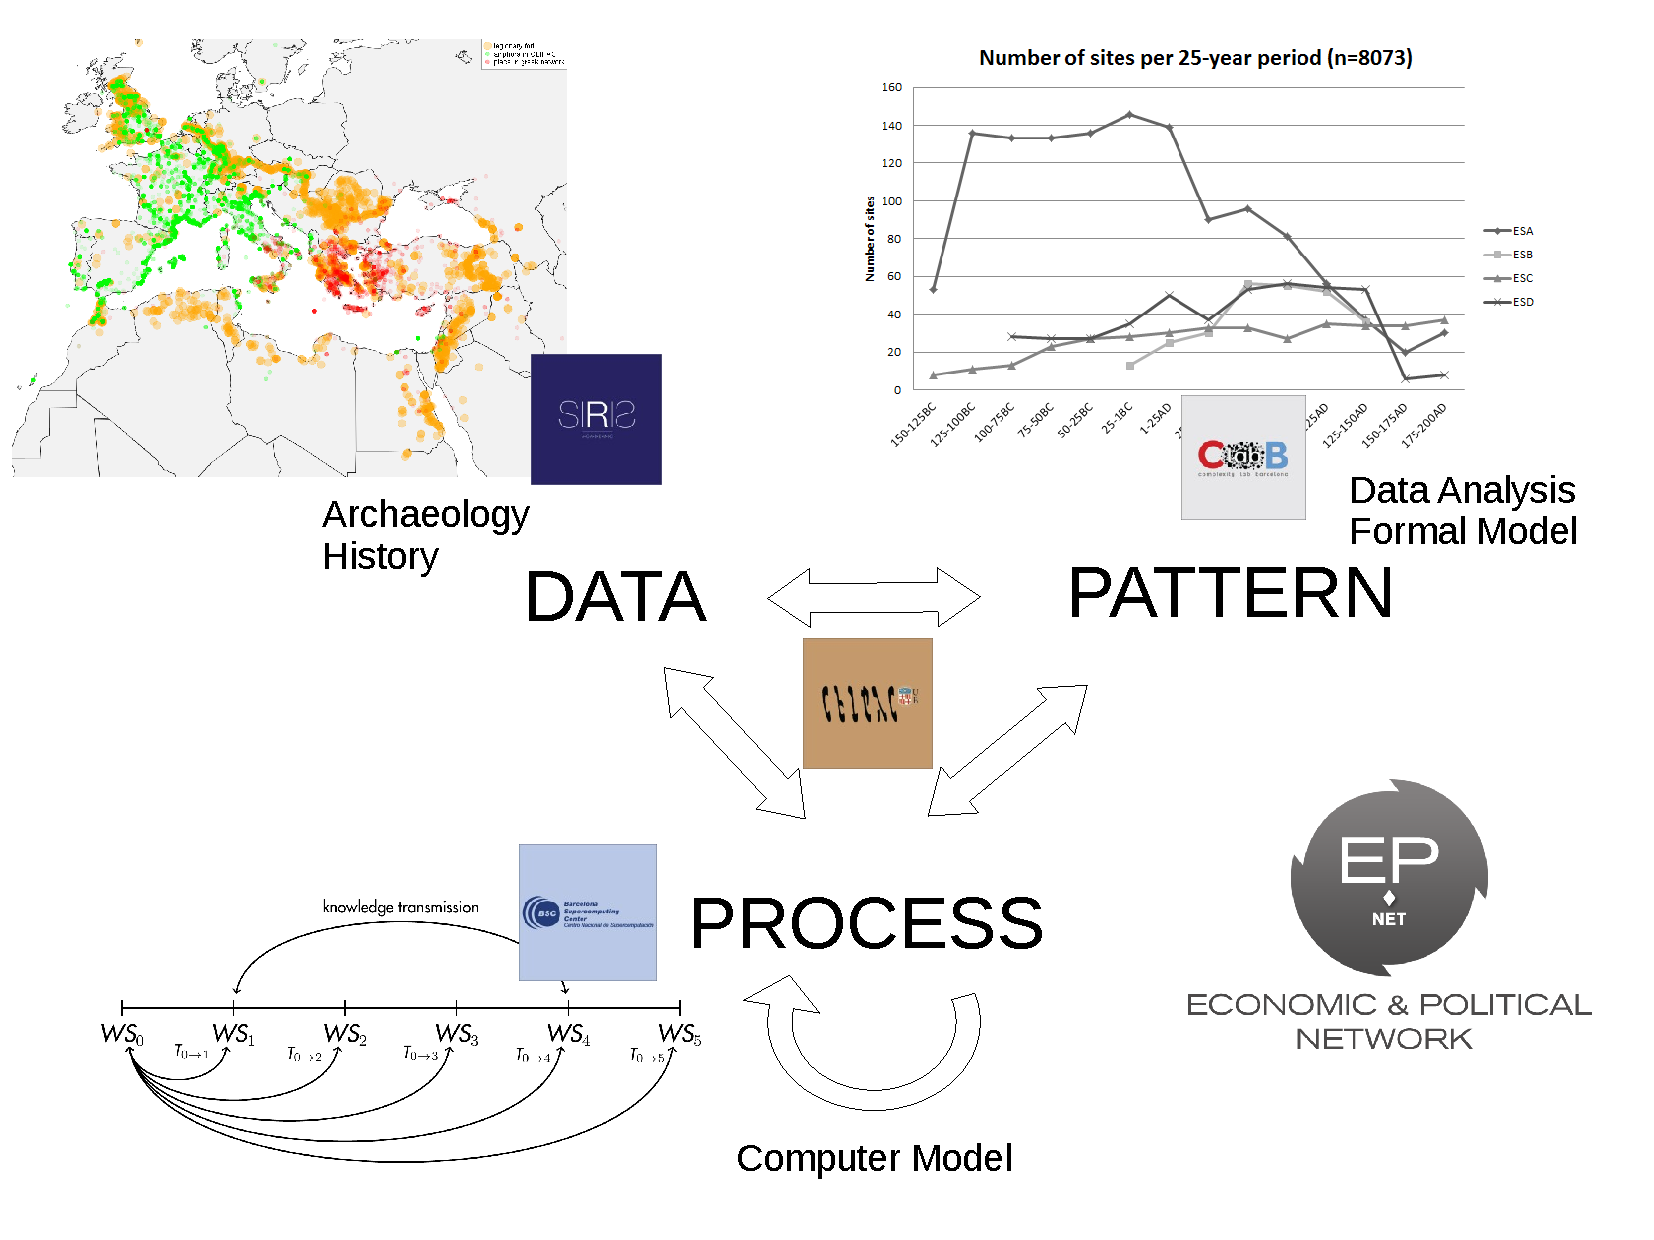
\includegraphics[width=\textwidth]{images/approach2.pdf}		
    \end{center}
    
\end{frame}

\begin{frame}
    \centering
    \Large
   Plan 
\end{frame}
\begin{frame}{Plan}
    \begin{enumerate}
	\item<1->Theoretical Exploration:\\ How economics value change the dynamics of Cultural Evolution (Computer Model vs Neutral Model) 
	\item<2-> Empirical Study:\\  Characterize an economy through socio-economic artefacts distribution, a case study the Roman Empire (Scaling Properties)
	\item<3-> Articulate the Theoretical Exploration \& the Empirical Observations
    \end{enumerate}

\end{frame}

\begin{frame}
    \centering
    \Large
    Theoretical Exploration
\end{frame}

\begin{frame}{A General Agent Based Framework }

     Two main components:
     \vfill
    \begin{enumerate}
	\item Trade side: Bartering Economy (Gintis 2009),
	\item Cultural side: ``copy the most successful'' (Bentley 2006).
    \end{enumerate}
    \begin{center}
	\includegraphics[width=.8\textwidth]{images/interaction}	
    \end{center}
\end{frame}
	

\begin{frame}{The Model}
	\begin{block}{1. The Economy \& the Barter Mechanism}
		\begin{itemize}
			\item $N$ goods
			\item $M$ Agent 
				$\left\{
					\begin{tabular}{@{}l@{}}
						a quantity of each Goods \\
						$N$ values attributed to each goods\\
					\end{tabular}
					\right.$
				\item Agents \emph{produce} one good and \emph{exchange} it to obtain the other goods.
				\item After the exchange, the agents \emph{consume} all goods 
			\end{itemize}
			Agent perform this 10 times and a scores is given to each of them.
		\end{block}
	\end{frame}

	\begin{frame}{The Model}
		\begin{block}{2. Cultural Mechanisms}
			\begin{itemize}
					\vfill
				\item Less successful agents \emph{copy} the most successful (Biased-Copy).
					\vfill
				\item Given a probability $\mu$ the value attributed to some goods is modified (Innovation/Mutation)
			\end{itemize}
		\end{block}
	\end{frame}
\begin{frame}{Experiments}
	\centering
	\textbf{Trade Model} \\Trade Mechanism + Success Biased Copy\\
	\vfill
	vs\\
	\vfill
	\textbf{Neutral Model}\\ Trade Mechanism + Random Copy\\
	 

\end{frame}


\section{Results}



\begin{frame}{Results: Economic Dynamic}
    \begin{figure}[!h]
	\centering
	\begin{tabular}{ c c}
	    Neutral Model & Trading Model \\
	    \includegraphics[width=5cm]{images/ScoreEvolutionForRandom-G3N500.pdf}
	    & 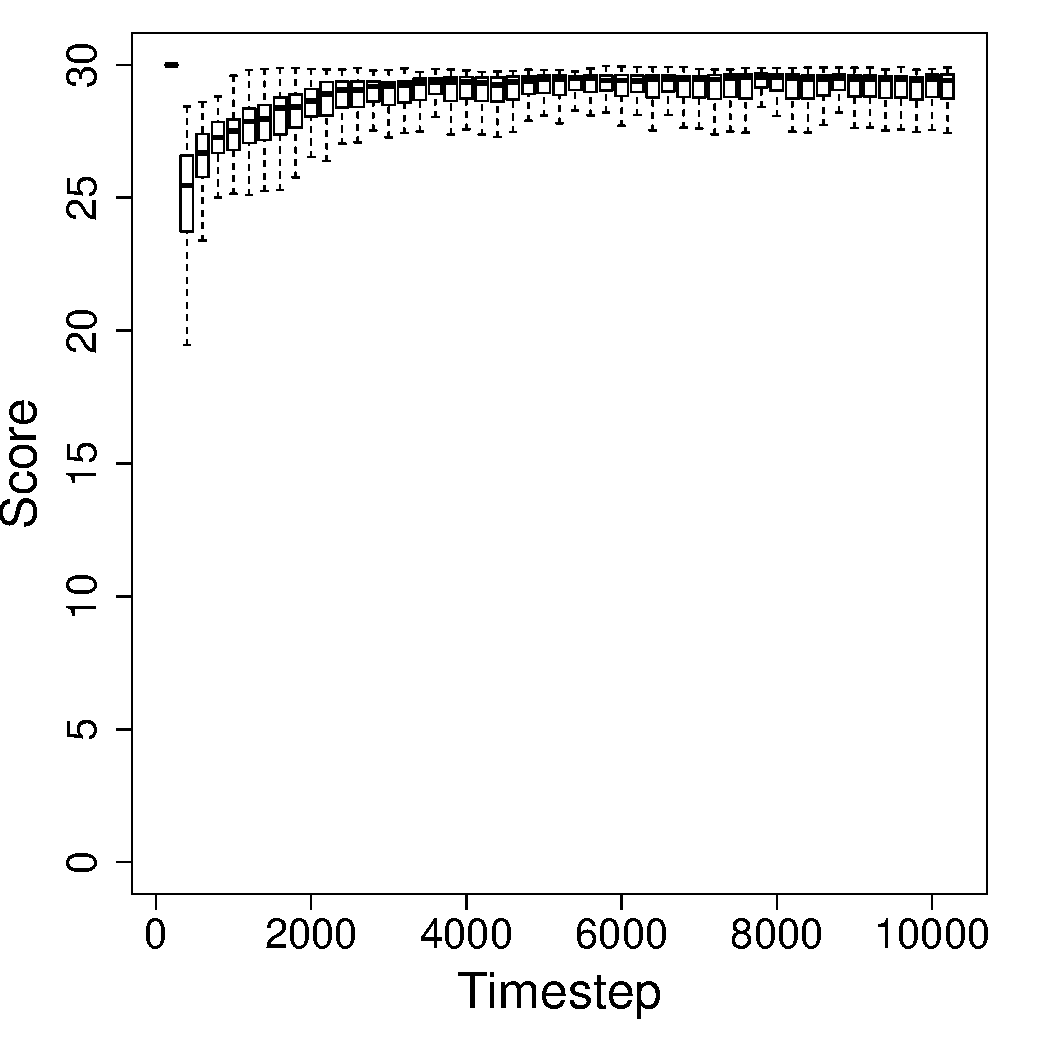
\includegraphics[width=5cm]{images/ScoreEvolutionForTrade-G3N500.pdf}

	\end{tabular}
	\caption{Evolution of the score within the two different models for two typical run with 500 agents and 3 goods evolving during 10000 timestep.}%%
	\label{fig:scoreEvol}
    \end{figure}
\end{frame}
    


\begin{frame}{Results: Economic Dynamics}
	\begin{figure}
	    \caption{Example for 3 goods and 500 agents}
	    \begin{columns}
		\column{.5\textwidth}
		\includegraphics[height=\textwidth]{images/ClearingPriceDistanceEvolutionForTrade-G3N500.pdf}\\
	    \end{columns}
		@~Equilibrium: personal values  $\rightarrow$ optimal (shared) values.
	\end{figure}
	
\end{frame}

\begin{frame}{Results: Frequency Distribution}
    \subsection*{Distribution of variant:}
    \begin{figure}[!h]
	\begin{center}
	    \begin{tabular}{ccc}
		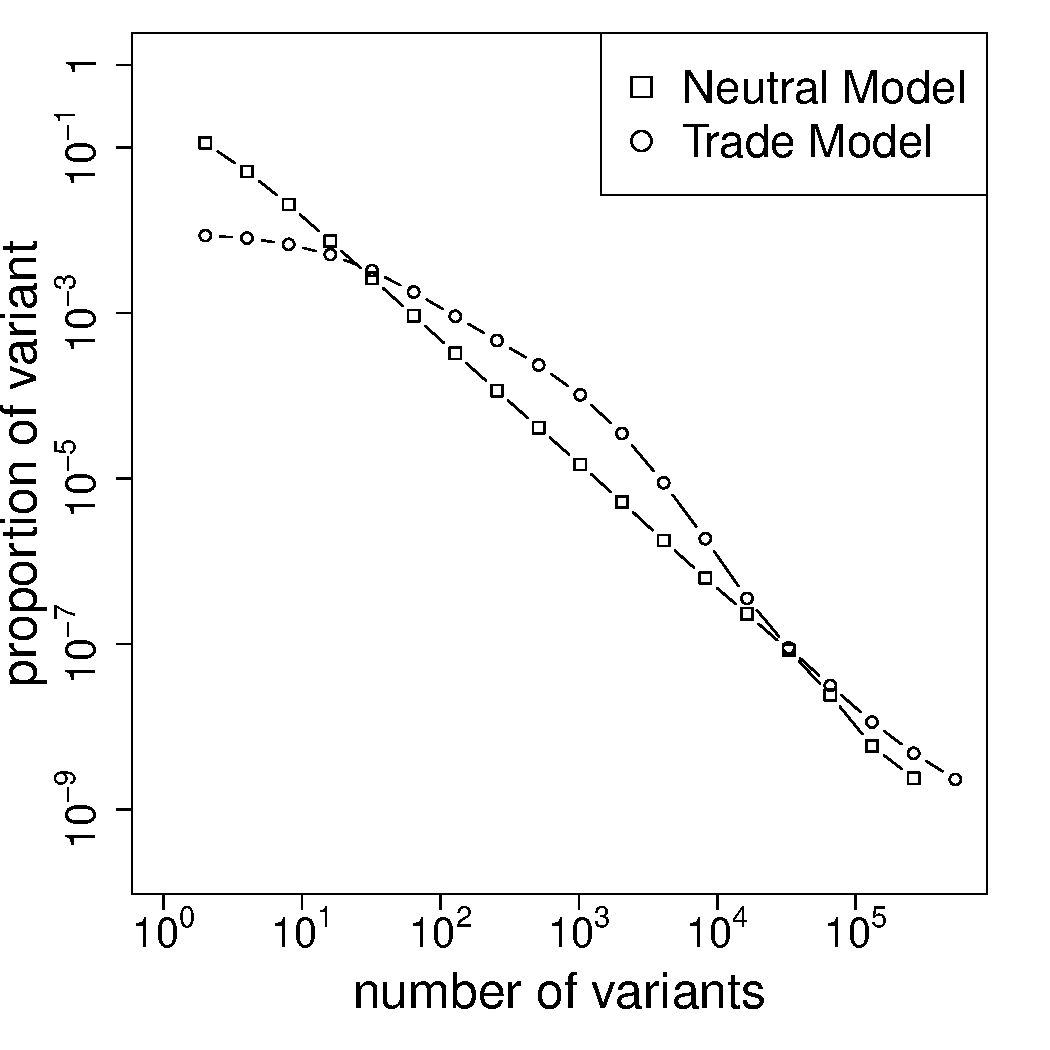
\includegraphics[width=5cm]{images/2SetupDistribA.pdf}\\
	    \end{tabular}

	\end{center}
	%\caption{Frequencies distribution, where each points represent the mean for 100 runs, for: a) the neutral and the trading models.  b) the neutral model and the trading model without the trading innovation process. c) the trade model and the trade model without the trading innovation process.}
    \end{figure}
\end{frame}

\begin{frame}{Next Objectives}
    \vfill
    Understand general dynamics and properties of such systems:
    \vfill
	\begin{itemize}
	\item Parameters fitting
    \vfill
	\item Different Cultural Mechanisms
    \vfill
	\item Different Trade Assumption
    \vfill
	\item Network Constraints
    \vfill
	\item \dots
    \vfill
	\end{itemize}
\end{frame}

\begin{frame}
    \centering
    \Large
   Empirical Studies 
\end{frame}
\begin{frame}{Empirical Studies}
	Characterize an economy through socio-economic artefacts distribution:\\
	\hspace{1cm} The need of strong proxy\\

	\vspace{.5cm}
    \uncover<2->{
	    Within EPNet:
	    
    \begin{itemize}
	\item Olive Oil production
	\item Wine production
	\item \ldots
    \end{itemize}}
    \uncover<3->{
	    \begin{alertblock}{Intuition}
		    Scaling properties of those indicators across cities to infer economic properties
	    \end{alertblock}
    }
\end{frame}

\begin{frame}{Scaling properties}
    \begin{figure}
	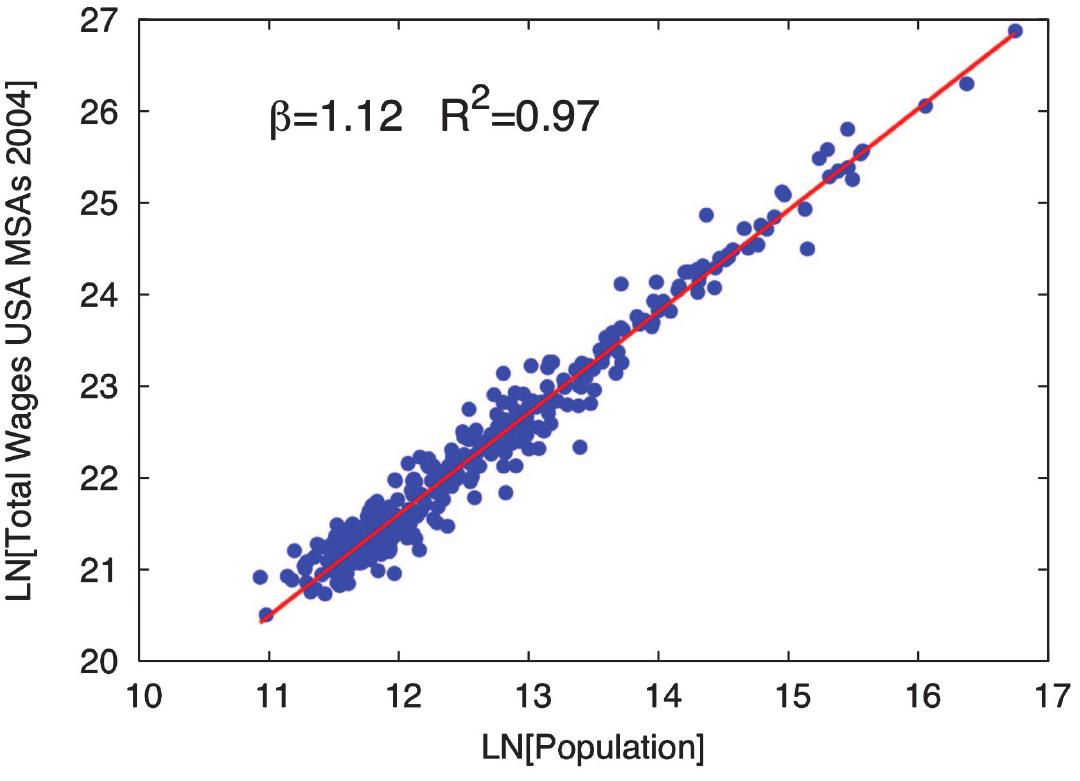
\includegraphics[width=.8\textwidth]{images/wageVsSize.jpg}
	\caption{ Bettencourt 2007}
    \end{figure}
\end{frame}



\begin{frame}
    \centering
    \Large
  Last Part
\end{frame}

\begin{frame}
 To what extent the theoretical model can explain the observed patterns?
    

\end{frame}

\begin{frame}{So far}
    \small
    \begin{itemize}
	\item Random Copy vs Economy-Biased Copy : WSC 15
	\item Social Network Impact on Economic dynamics: Complenet \& CAA 16
	\item  Scaling Law and Cities: DACAS1 16
	\item  Model and Computer Sim in History \&  Archaeology: MS7 16
    \end{itemize}
    
\end{frame}

\begin{frame}
    %{Case Study}
	\begin{center}
		\Large
    Thank for coming \& for you attention!\\
		\vspace{1cm}
%		What was the nature of Roman economy?\\
		\includegraphics[width=2cm]{images/LOGO-ERC.jpg} \hfil	\includegraphics[width=3cm]{images/epnetLogo.png}\\
	\end{center}


\end{frame}

\end{document}


